\chapter{Characterising SDE linearisations: the numerics}

\section{Direct verification of bound}\label{sec:numerics}

This section will validate the theory presented in \Cref{sec:theory}, by considering three examples each leading to a different form of the strong error bound \eqref{eqn:main_ineq}.
For each example SDE, we first demonstrate heuristically that the solution converges to the limiting distribution described by \Cref{thm:limit_sol}, and then verify the error bound in \Cref{thm:main} directly by considering a range of values for the noise scale \(\epsilon\) and initial condition uncertainty \(\delta\).

% To compute the limiting covariance matrix, we solve the differential equation \eqref{eqn:pi_ode} numerically, which is more convenient than evaluating the explicit expressions \eqref{eqn:pi_expl_eqn} directly.
% The covariance equation \eqref{eqn:pi_ode} is solved jointly with the deterministic state equation \eqref{eqn:pi_ode} using the hybrid method proposed by \citet{Mazzoni_2008_ComputationalAspectsContinuous}, which combines a Taylor-Heun approximation with a Gauss-Legendre and ensures that the numerical solution of the covariance equation is symmetric and positive semi-definite while maintaining computational efficiency.

% \rev{This is to highlight both the validity and computability of this alternative expression.}
% All necessary flow map data is obtained by directly solving \eqref{eqn:ode_det} numerically, with the standard Euler scheme.
% The flow map gradients required for computing the covariance matrix with \eqref{eqn:sigma_calc} are calculated via a star-grid finite-difference approximation, using a spatial resolution of \(0.001\).


All simulations in this section were generated using the Julia programming language \cite{BezansonEtAl_2017_JuliaFreshApproach}, with implementations of the ordinary and stochastic differential equation numerical solvers provided by the DifferentialEquations.jl package \cite{RackauckasNie_2017_DifferentialEquationsJlPerformant}.
The code is available at \href{https://github.com/liamblake/explicit-characterisation-sde-linearisation}{github.com/liamblake/explicit-characterisation-sde-linearisation}.




\subsection{Nonlinear dynamics, additive noise}\label{sec:numerics_nonlinear}
Consider the following SDE in 1D;
\begin{equation}\label{eqn:sine_sde}
	\dif y_t^{(\epsilon)} = \sin\!\left(y_t^{(\epsilon)}\right)\dif t + \epsilon \dif W_t.
\end{equation}
The deterministic system corresponding to \eqref{eqn:sine_sde} has solution
\[
	F_0^t\!\left(x_0\right) = 2\arctan\left(e^{-t}\tan\left(\frac{x_0}{2}\right)\right).
\]

To explore the impact of initial condition uncertainty, we consider the univariate Gaussian initial condition \(y_0 = x \sim \Gauss{\mu, \rho^2}\), where the mean \(\mu\) is specified and the standard deviation \(\rho\) is a non-negative scaling parameter.
We linearise about the deterministic trajectory \(F_0^t\!\left(\mu\right)\) originating from the mean, that is choosing \(\mu\) as our reference point.
This ensures that for any \(r \geq 0\)
\begin{equation}\label{eqn:num_gauss_init}
    \delta_r = \avg{\abs{x - \mu}^r} = M_r \rho^r.
\end{equation}
where \(M_r\) is as defined in \eqref{eqn:gauss_dist_bound}.
This property of the univariate Gaussian distribution allows us to easily control the uncertainty in the initial condition and verify the bounds; by sending the parameter \(\rho\) to zero we ensure that \(\delta_r\) approaches zero also.
The linearised solution then follows a Gaussian distribution, specifically
\begin{equation}\label{eqn:num_linear_sol}
	l_t^{(\epsilon)} \isGauss{F_0^t\!\left(x_0\right), \, \nabla F_0^t\!\left(x_0\right)^2\rho^2 + \Sigma_0^t\!\left(x_0\right)}.
\end{equation}
where \(\Sigma_0^t\!\left(x_0\right)\) is computed by solving \eqref{eqn:pi_ode} numerically.
To validate the strong error bound predicted by \Cref{thm:main} under the Gaussian initial condition \eqref{eqn:num_gauss_init}, define for \(r \geq 1\) the error measure
\begin{equation}
	E_r\!\left(\epsilon, \rho\right) \coloneqq \frac{1}{N}\sum_{i=1}^N{\norm{\hat{y}_{i}^{(\epsilon)} - \hat{l}_i^{(\epsilon)}}^r},
	\label{eqn:strong_err_mc_estimate}
\end{equation}
which is a Monte-Carlo estimator of the right-hand side of \eqref{eqn:main_ineq}, where \(\hat{y}_1^{(\epsilon)},\dotsc, \hat{y}_N^{(\epsilon)}\) and \(\hat{l}_1^{(\epsilon)},\dotsc, \hat{l}_N^{(\epsilon)}\) are \(N\) numerical samples of the solutions to SDE \eqref{eqn:sde_y} and the linearisation \eqref{eqn:linear_sde_inform} respectively.

The linearised equation is then
\begin{equation}
	\dif l_t^{(\epsilon)} = \left[F_0^t\!\left(\mu\right) + \cos\!\left(F_0^t\!\left(\mu\right)\right)\left(l_t^{(\epsilon)} - F_0^t\!\left(\mu\right)\right)\right]\dif t + \epsilon \dif W_t, \quad l_0^{(\epsilon)} \isGauss{\mu, \rho^2}.
    \label{eqn:sine_linear}
\end{equation}
In this example, we take \(\mu_0 = 0.5\) and consider the solutions of \eqref{eqn:sine_sde} and \eqref{eqn:sine_linear} at time \(t = 1.5\).
We generate samples of \ref{eqn:sine_sde} and \eqref{eqn:sine_linear} jointly (that is, using the same realisations of the Wiener process \(W_t\)) using the stochastic Runge-Kutta scheme SRI \cite{Rossler_2010_RungeKuttaMethodsStrong} with an adaptive step size.

\begin{figure}
    \centering
    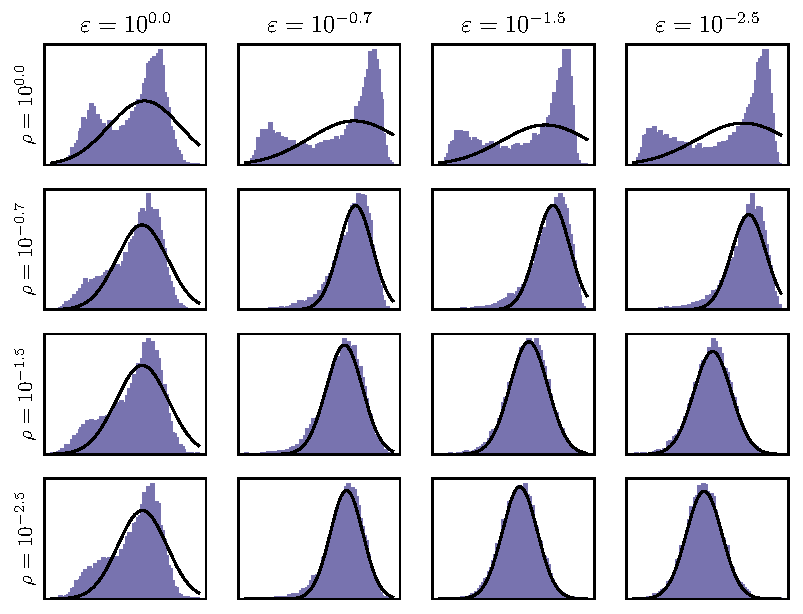
\includegraphics[width=\textwidth]{chp04_paper_numerics/figures/sine/selected_hists.pdf}
		\caption{Histograms of stochastic samples of \eqref{eqn:sine_sde}, subject to the Gaussian initial condition \eqref{eqn:num_gauss_init}, for varying initial uncertainty scale \(\epsilon\) and ongoing uncertainty scale \(\rho\).
		The distribution of the corresponding solution \eqref{eqn:num_linear_sol} to the linearised equation is overlaid in black.}
    \label{fig:sine_hists}
\end{figure}

In \Cref{fig:sine_hists}, we show histograms of \(N = 10000\) samples of the nonlinear SDE \eqref{eqn:sine_sde} and the corresponding probability density function of the linearised solution, for different combinations of \(\epsilon\) and \(\rho\).
Even when the ongoing noise is small, the nonlinearity of the drift term means that a large initial uncertainty results in a non-Gaussian distribution.
However, in situations where both the initial and ongoing uncertainties are small, the Gaussian solution to the linearised equation provides a reasonable approximation. %\lb{Reconsider what I'm saying here - probably also need to discuss quickly what is going on when \(\rho\) is small but \(\epsilon\) is large.}
In the limit of both small initial (\(\rho \to 0\)) and small ongoing (\(\epsilon \to 0\)) uncertainty (towards the bottom right), we see that the distribution of the samples approach the Gaussian density of the linearisation solution, matching the understanding that the linearisation approximation is ``reasonable'' for small noise regimes.

Since the drift term is nonlinear and the noise is additive in \eqref{eqn:sine_sde}, the bound predicted by \Cref{thm:main} has the form
\[
	\avg{\norm{y_t^{(\epsilon)} - l_t^{(\epsilon)}}^r} \leq D_1\left(r, t\right)\epsilon^{2r} + M_{2r}D_2\!\left(r,t\right)\rho^{2r}.
\]
where we have \(K_{\nabla\nabla u} = 1\) and \(K_{\nabla\sigma} = 0\).
We directly validate the \emph{form} of this bound (as a function of \(\epsilon\) and \(\rho\)) in \Cref{fig:sine_delta_eps_lines}, by computing \(E_1\) using samples for each pair of \(\epsilon\) and \(\rho\) values.
In \Cref{fig:sine_eps_lines}, we demonstrate the relationship between \(E_1\) and the ongoing uncertainty \(\epsilon\) for several different fixed values of \(\rho\), each corresponding to a different colour.
A least squares estimate of a line of best fit of the form \(E_1 = \beta_0 + \beta_1 \epsilon^2 \), for fixed coefficients \(\beta_0\) and \(\beta_1\), is fitted to the observed errors (in untransformed space) to verify the scaling of our bound in \Cref{thm:main}.
We see that the line of best fit accurately matches the observed values of \(E_1\), verifying that \(E_1\) is in fact scaling with \(\epsilon^2\) as predicted.
\Cref{fig:sine_delta_lines} provides a similar demonstration between \(E_1\) and the initial uncertainty \(\rho\), where now each colour corresponds to a different fixed value of \(\epsilon\).
We again fit lines of the form \(E_1 = \beta_0 + \beta_1 \rho^2\) to verify the scaling of the bound, and see that the lines match the observed values of \(E_2\).
Thus, we have also validated that \(E_1\) scales with \(\rho^2\), as expected from \Cref{thm:main}.
Additional plots verifying the scaling for \(E_2\), \(E_3\) and \(E_4\) are provided in the supplementary materials.

\begin{figure}
	\begin{center}
		\begin{subfigure}{\textwidth}
			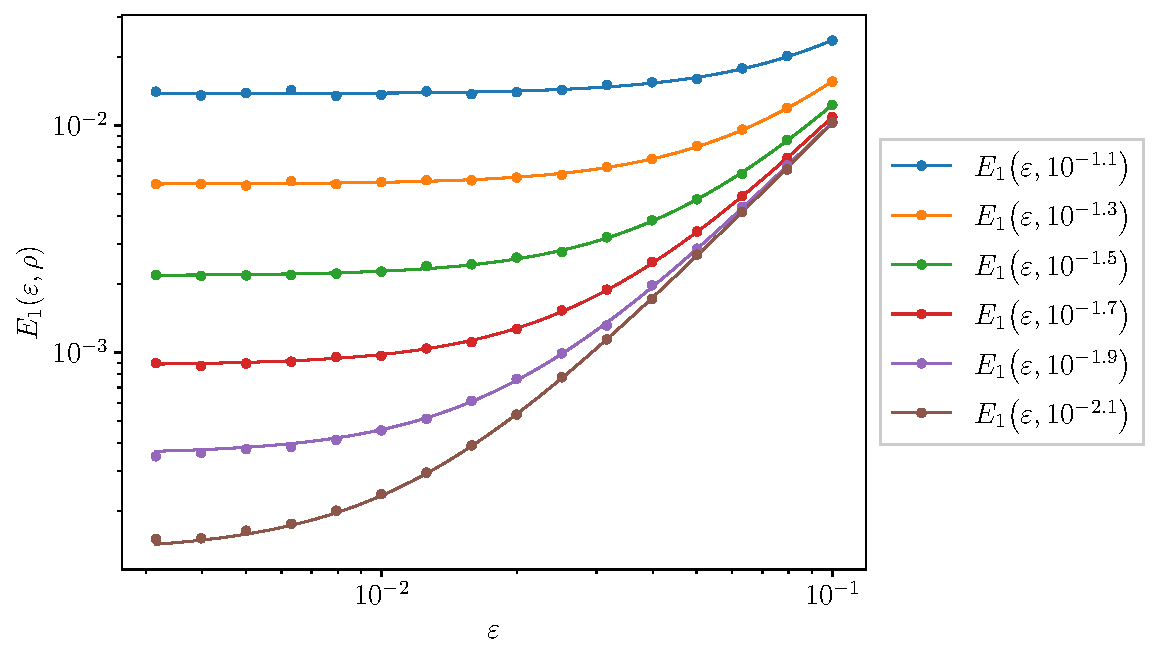
\includegraphics[width=\textwidth]{chp04_paper_numerics/figures/sine/str_err_eps_r_1.0_log.pdf}
			\caption{Estimates of the strong error (with \(r = 1\)) in linearising \eqref{eqn:sine_sde} with \eqref{eqn:sine_linear}, for varying ongoing uncertainty parameter \(\epsilon\).
   Each colour corresponds to a different value of the initial uncertainty parameter \(\rho\).
   A (least squares) line of best fit of the form \(\beta_0 + \beta_1 \epsilon^2\) is included in the corresponding colour.}
			\label{fig:sine_eps_lines}
		\end{subfigure}
		\begin{subfigure}{\textwidth}
			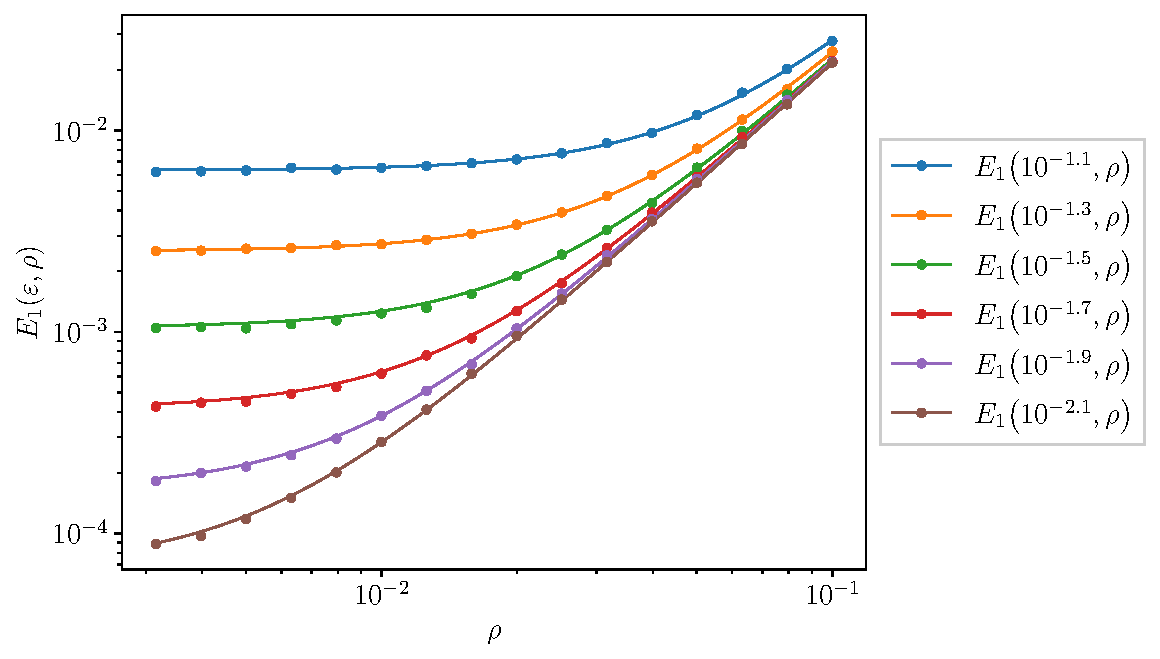
\includegraphics[width=\textwidth]{chp04_paper_numerics/figures/sine/str_err_rho_r_1.0_log.pdf}
			\caption{Estimates of the strong error (with \(r = 1\)) for varying initial uncertainty parameter \(\rho\).
			Each colour corresponds to a different value of the ongoing uncertainty parameter \(\epsilon\).
			A (least squares) line of best fit of the form \(\beta_0 + \beta_1 \rho^2\) is included in the corresponding colour.}
			\label{fig:sine_delta_lines}
		\end{subfigure}
		\caption{Validation of the theoretical bound predicted by \Cref{thm:main}, when \(r = 1\), on numerical realisations of the solution to the 1D example \eqref{eqn:sine_sde}.}
		\label{fig:sine_delta_eps_lines}
	\end{center}
\end{figure}

\subsection{Linear dynamics, multiplicative noise}\label{sec:numerics_multiplicative}
Now consider the following SDE with multiplicative noise in 1D:
\begin{equation}
	\dif y_t^{(\epsilon)} = \frac12 y_t^{(\epsilon)}\dif t + \varepsilon \cos\!\left(y_t^{(\epsilon)}\right) \dif W_t.
		\label{eqn:1d_mult}
\end{equation}
The corresponding deterministic system is linear and has solution
\begin{equation}
F_0^t\!\left(x_0\right) = \exp\!\left(\frac{t}{2}\right) x_0.
	\label{eqn:1d_mult_det_sol}
\end{equation}
As with the previous example in \Cref{sec:numerics_nonlinear}, we take the Gaussian initial condition \eqref{eqn:num_gauss_init} with variance \(\rho^2\) and linearised \eqref{eqn:1d_mult} about the initial mean \(\mu\).
The linearised equation is then
\begin{equation}
	\dif l_t^{(\epsilon)} = \frac12 l_t^{(\epsilon)}\dif t + \epsilon \cos\!\left(\exp\left(\frac{t}{2}\right)\mu\right) \dif W_t, \quad l_0^{(\epsilon)} \sim \Gauss{\mu, \rho^2},
	\label{eqn:1d_mult_linear}
\end{equation}
with Gaussian solution \eqref{eqn:num_linear_sol}.
We take the initial point \(\mu = 2\) and consider the solutions at time \(t = 1\).
To generate numerical realisations of the solutions to \eqref{eqn:1d_mult} and \eqref{eqn:1d_mult_linear} with the same realisations of \(W_t\), we use the same set-up as in the previous example.

In \Cref{fig:sine_hists}, we show histograms of \(N = 10000\) samples of the multiplicative noise SDE \eqref{eqn:1d_mult} and the corresponding probability density function of the linearised solution, for different combinations of \(\epsilon\) and \(\rho\).
We again see that in the limit of both small initial and small ongoing uncertainty (towards the bottom right), we see that the distribution of the samples approach the Gaussian density of the linearisation solution.

\begin{figure}
	\begin{center}
    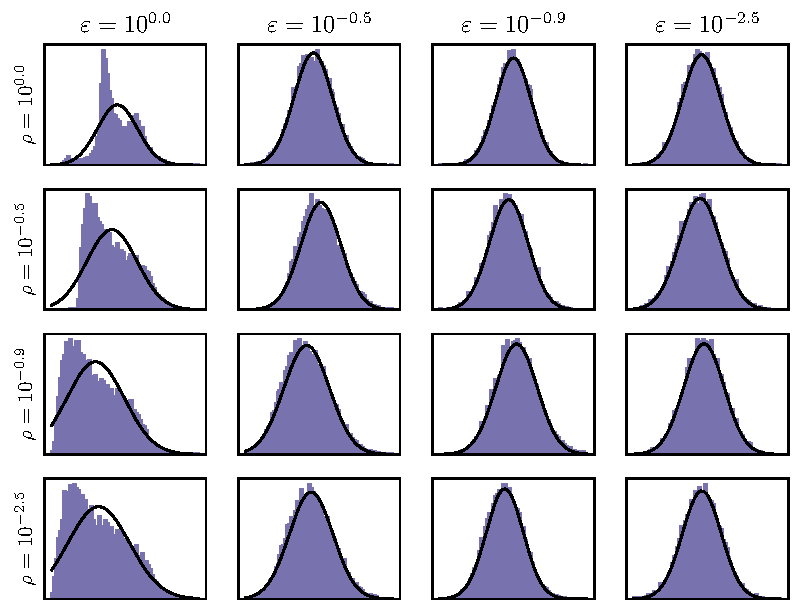
\includegraphics[width=\textwidth]{chp04_paper_numerics/figures/multiplicative/selected_hists.pdf}
		\caption{The same arrangement as \Cref{fig:sine_hists}, but for the 1D multiplicative noise SDE \eqref{eqn:1d_mult}.}
		\label{fig:1d_mult_hists}
	\end{center}
\end{figure}

Since the drift term is linear and the noise multiplicative in \eqref{eqn:1d_mult}, the bound predicted by \Cref{thm:main} has the form
\[
	\avg{\norm{y_t^{(\epsilon)} - l_t^{(\epsilon)}}^r} \leq D_1\left(r, t\right)\epsilon^{2r} + M_{r}D_3\!\left(r,t\right)\epsilon^r\rho^{r},
\]
where we have \(K_{\nabla\nabla u} = 0\) and \(K_{\nabla\sigma} = 1\).
In \Cref{fig:multiplicative_delta_eps_lines}, we again validate the form of this bound (for \(r = 1\); results for additional values of \(r\) are provided in the supplementary material) by approximating the left-hand side with \(E_1\) computed from realisations of the solution to \eqref{eqn:1d_mult} and the linearisation \eqref{eqn:1d_mult_linear}.
For each fixed value of the initial uncertainty \(\rho\), in \Cref{fig:multiplicative_eps_lines}, we fit a line of best fit of the form \(\beta_1 \epsilon + \beta_2 \epsilon^2\) to validate that the strong error scales as predicted.
Similarly, in \Cref{fig:multiplicative_eps_lines} we fit a line of best fit of the form \(\beta_0 + \beta_1 \rho\) and validate that the linearisation error follows this scaling.

\begin{figure}
	\begin{center}
		\begin{subfigure}{\textwidth}
			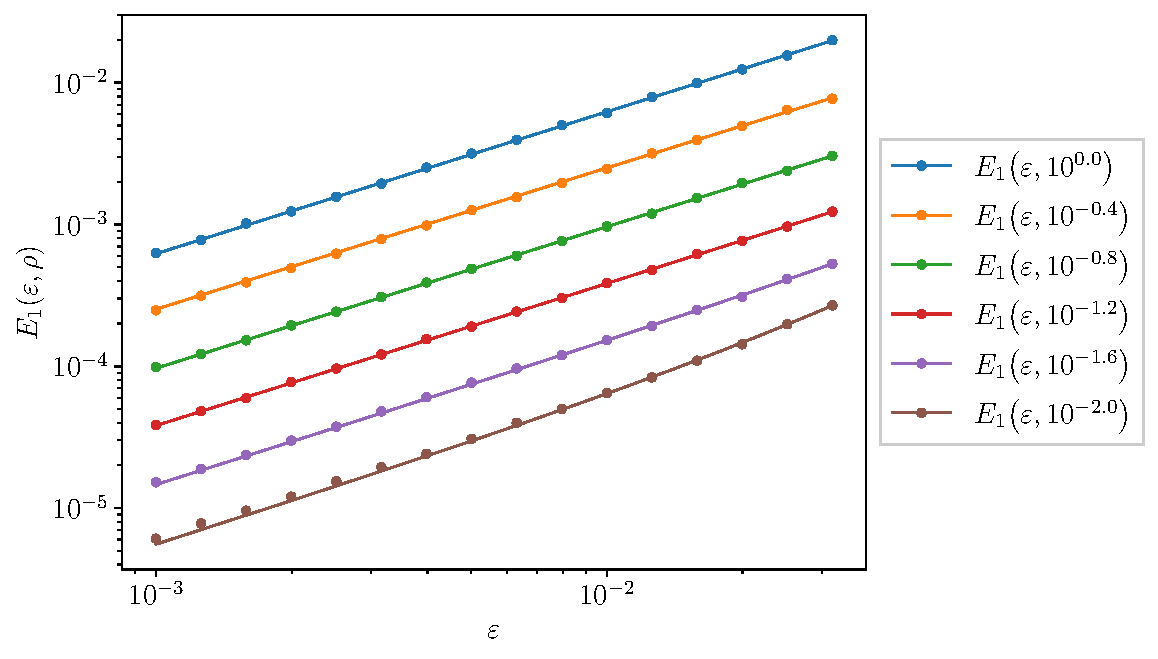
\includegraphics[width=\textwidth]{chp04_paper_numerics/figures/multiplicative/str_err_eps_r_1.0_log.pdf}
			\caption{Estimates of the strong order (with \(r = 1\)) for varying ongoing uncertainty parameter \(\epsilon\).
			Each colour corresponds to a different value of the initial uncertainty parameter \(\rho\).
			A (least squares) line of best fit of the form \(\beta_1 \epsilon + \beta_2 \epsilon^2\) is included in the corresponding colour.}
			\label{fig:multiplicative_eps_lines}
		\end{subfigure}
		\begin{subfigure}{\textwidth}
			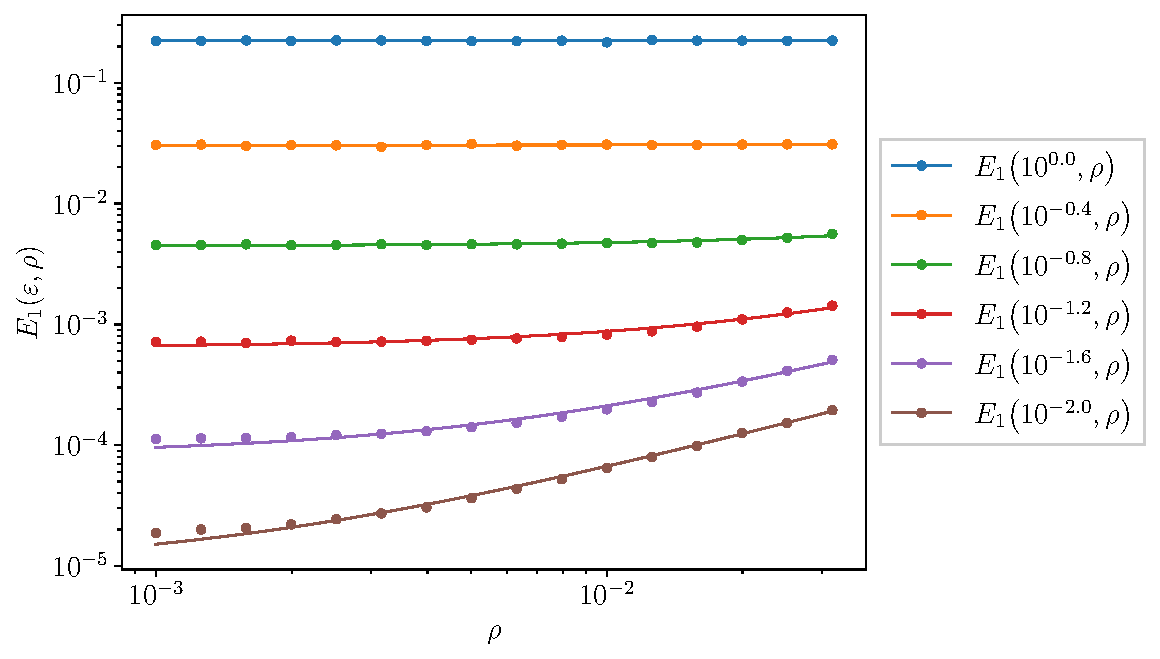
\includegraphics[width=\textwidth]{chp04_paper_numerics/figures/multiplicative/str_err_rho_r_1.0_log.pdf}
			\caption{Estimates of the strong order (with \(r = 1\)) for varying initial uncertainty parameter \(\rho\).
			Each colour corresponds to a different value of the ongoing uncertainty parameter \(\epsilon\).
			A (least squares) line of best fit of the form \(\beta_0 + \beta_1 \rho\) is included in the corresponding colour.}
			\label{fig:multiplicative_delta_lines}
		\end{subfigure}
		\caption{Validation of the theoretical bound predicted by \Cref{thm:main}, when \(r = 1\), on numerical realisations of the solution to the 1D example \eqref{eqn:1d_mult}.}
		\label{fig:multiplicative_delta_eps_lines}
	\end{center}
\end{figure}

\subsection{Fixed initial condition}\label{sec:numerics_2d}
In our final example, we consider a two-dimensional model and a fixed initial condition, to validate the results presented in \Cref{sec:theory_fixed}.
Following the example in Chapter 5 of \cite{SamelsonWiggins_2006_LagrangianTransportGeophysical}, we consider an unsteady meandering jet in two dimensions, which may serve as an idealised model of geophysical Rossby waves.
The velocity field for \(y \equiv \left(y_1, y_2\right)\) is given by \cite{SamelsonWiggins_2006_LagrangianTransportGeophysical}
\begin{equation}
	u\!\left(y, t\right) = \begin{bmatrix}
		c - A\sin\!\left(Ky_1\right)\cos\!\left(y_2\right) + \oldepsilon_{\mathrm{mj}} l_1\sin\!\left(k_1\left(y_1 - c_1 t\right)\right)\cos\!\left(l_1 y_2\right) \\
		AK\cos\!\left(Ky_1\right)\sin\!\left(y_2\right) + \oldepsilon_{\mathrm{mj}} k_1\cos\!\left(k_1\left(y_1 - c_1t\right)\right)\sin\!\left(l_1 y_2\right)
	\end{bmatrix}.
 \label{eqn:jet_ex}
\end{equation}
The velocity field describes a kinematic travelling wave with deterministic oscillatory perturbations in a co-moving frame.
Here, \(A\) is the amplitude and \(c\) is the phase speed of the primary wave, and \(K\) is the wavenumber in the \(y_1\)-direction.
The oscillatory perturbation has amplitude \(\oldepsilon_{\mathrm{mj}}\), phase speed \(c_1\) (in the co-moving frame), and wavenumbers \(k_1\) and \(l_1\) in the \(y_1\)- and \(y_2\)-directions respectively.
Throughout, we take the parameter values \(c = 0.5\), \(A = 1\), \(K = 4\), \(l_1 = 2\), \(k_1 = 1\), \(c_1 = \pi\), and \(\oldepsilon_{\mathrm{mj}} = 0.3\).
For these values, the flow consists of a meandering jet with vortex structures within the meanders, and a chaotic zone
which influences the fluid transfer between the jet and the vortices.

We introduce multiplicative noise by considering stochastic perturbations to primary amplitude \(A\) and phase speed \(c\), which we model with the respective components of a \(2\)-dimensional Wiener process \(W_t = \left(W_t^{(1)}, W_t^{(2)}\right)^{\T}\).
Then, we specify the diffusion term as
\begin{equation}
	\sigma\!\left(y,t\right) = \begin{bmatrix}
		1 & \sin\!\left(Ky_1\right)\cos\!\left(y_2\right) \\
		0 & K\cos\!\left(Ky_1\right)\sin\!\left(y_2\right)
	\end{bmatrix}.
	\label{eqn:jet_ex_sigma}
\end{equation}

To compute the Gaussian distribution \eqref{eqn:linear_gauss_sol} of the linearised solution, we again solve \eqref{eqn:pi_ode} numerically with initial condition \(\Sigma_0^t\!\left(x_0\right) = O\).
Specifically, \eqref{eqn:pi_ode} is solved jointly with the deterministic state equation \eqref{eqn:ode_det} using the hybrid method proposed by \citet{Mazzoni_2008_ComputationalAspectsContinuous}.
This hybrid method combines a Taylor-Heun approximation with a Gauss-Legendre one and ensures that the numerical solution of the covariance equation is symmetric and positive semi-definite while maintaining computational efficiency.

To again numerically estimate the left-hand side of \eqref{eqn:main_ineq}, we use the Monte-Carlo estimator
\[
	E_r\!\left(\epsilon\right) \coloneqq \frac{1}{N}\sum_{i=1}^N{\norm{\hat{y}_i^{(\epsilon)} - \hat{l}_i^{(\epsilon)}}^r}.
\]
We consider the fixed initial condition \(x_0 = \left(0, 1\right)\) and the prediction of the model at time \(t = 1\).
% For each value of \(\epsilon\) considered, we use the Euler-Maruyama method \cite{KloedenPlaten_1992_NumericalSolutionStochastic} to generate \(N = 10000\) independent realisations of the solutions to \eqref{eqn:sde_y} and \eqref{eqn:limit_sde}.
% A step size of \(\delta t = 10^{-4}\) is used to ensure that numerical error does not dominate over the theoretical predictions.
% These solution samples are generated with the \emph{same} realisations of the Wiener process increments \(W_{t + \delta t} - W_t \sim \mathcal{N}\left(0, \delta t I_n\right)\).
% For each realisation of \(y_t^{(\epsilon)}\), a corresponding realisation of the scaled deviation \(z_t^{(\epsilon)}(x)\) is computed.
% In the following, let \(\hat{z}_1^{(\epsilon)},\hdots, \hat{z}_N^{(\epsilon)}\) and \(\hat{z}_1,\hdots, \hat{z}_N\) denote the \(N\) realisations of \(z_t^{\left(\epsilon\right)}(x)\) and \(z_t(x)\) respectively.


\Cref{fig:y_hists} shows the resulting simulations of \(y_t^{(\epsilon)}\) for four different values of \(\epsilon\).
The realisations are binned as a histogram and bin counts are normalised, to provide an empirical estimate of the probability density function of \(y_t^{(\epsilon)}\).
Superimposed (in solid black) are the first, second and third standard-deviation contours of the probability density function of the Gaussian distribution that solves the linearised equation.
The first three standard-deviation levels of the \(2\times 2\) sample covariance matrix of the realisations of \(y_t^{(\epsilon)}\), are also overlaid (in dashed blue).
As \(\epsilon\) decreases towards \(0\), the samples increasingly resemble a Gaussian distribution, and both the mean and covariance coincide with the corresponding limits.

\begin{figure}
	\begin{center}
        % 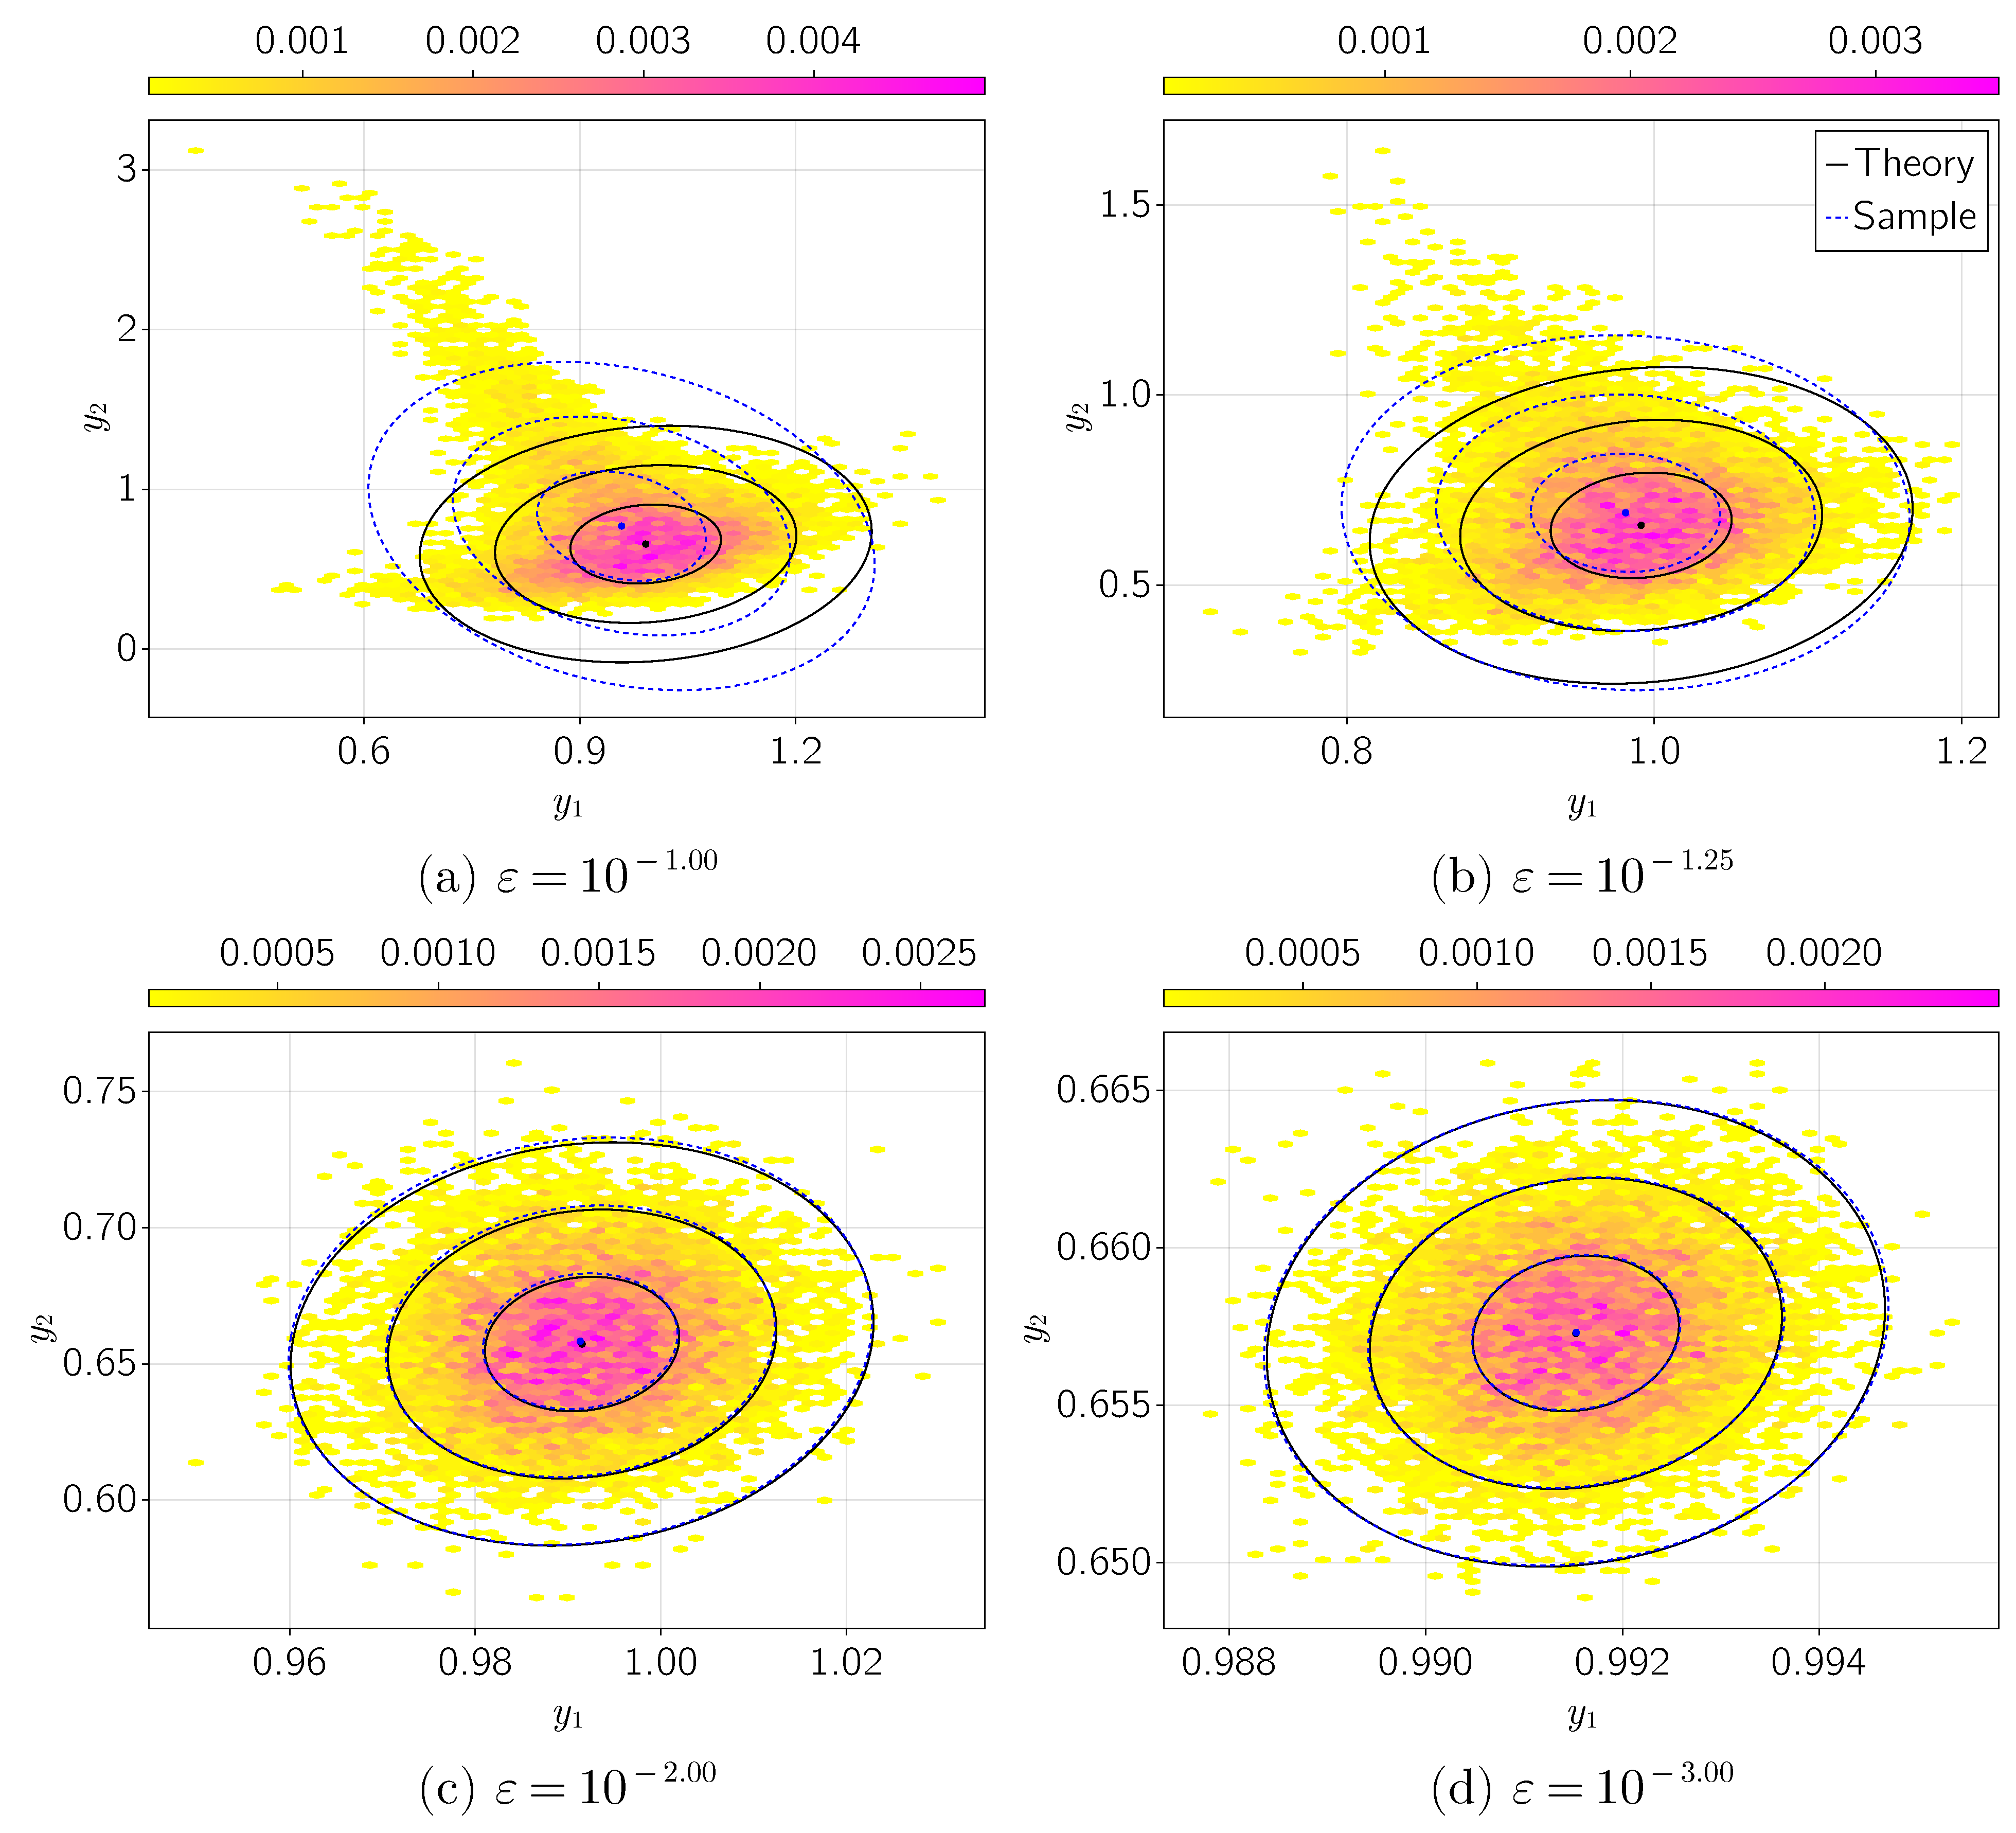
\includegraphics[width=\textwidth]{figures/y_histogram.pdf}
				% \td{Increase size/clarity of points at centre of contours}
		\begin{subfigure}{0.49\textwidth}
			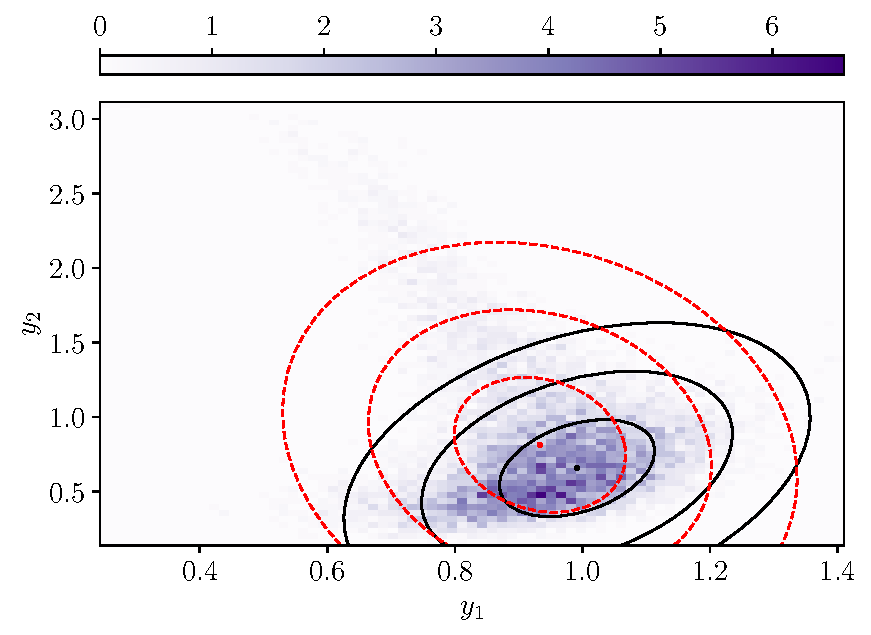
\includegraphics[width=\textwidth]{chp04_paper_numerics/figures/rossby/hist_0.1.pdf}
			\caption{\(\epsilon = 10^{-1}\)}
			\label{fig:y_hists_a}
		\end{subfigure}
		\begin{subfigure}{0.49\textwidth}
			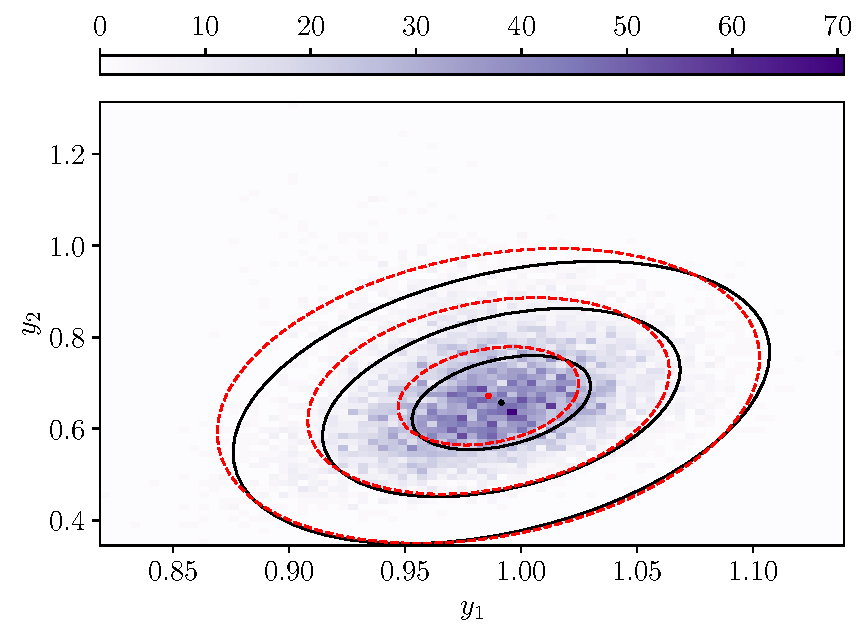
\includegraphics[width=\textwidth]{chp04_paper_numerics/figures/rossby/hist_0.03162277660168379.pdf}
			\caption{\(\epsilon = 10^{-1.5}\)}
			\label{fig:y_hists_b}
		\end{subfigure}
		\begin{subfigure}{0.49\textwidth}
			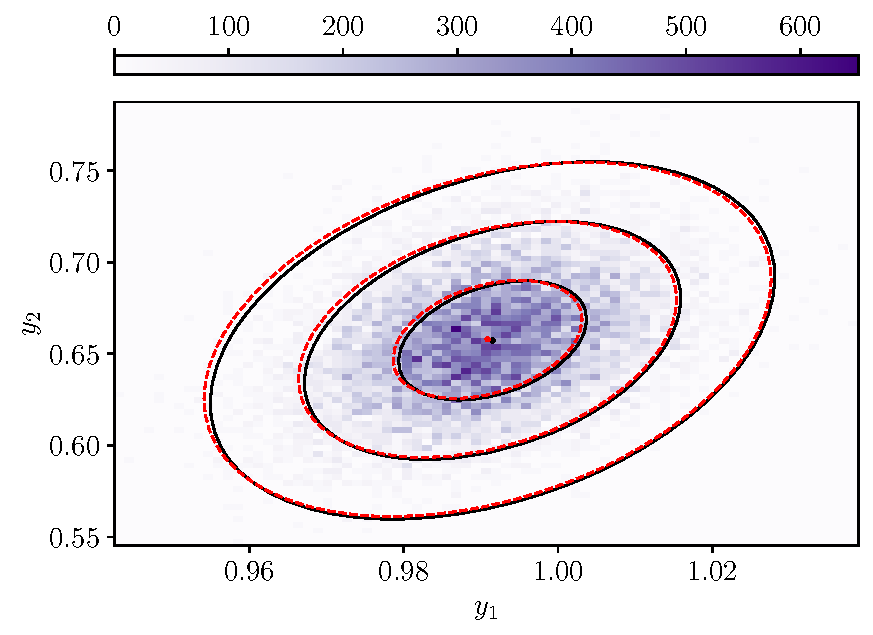
\includegraphics[width=\textwidth]{chp04_paper_numerics/figures/rossby/hist_0.010000000000000002.pdf}
			\caption{\(\epsilon = 10^{-2}\)}
			\label{fig:y_hists_c}
		\end{subfigure}
		\begin{subfigure}{0.49\textwidth}
			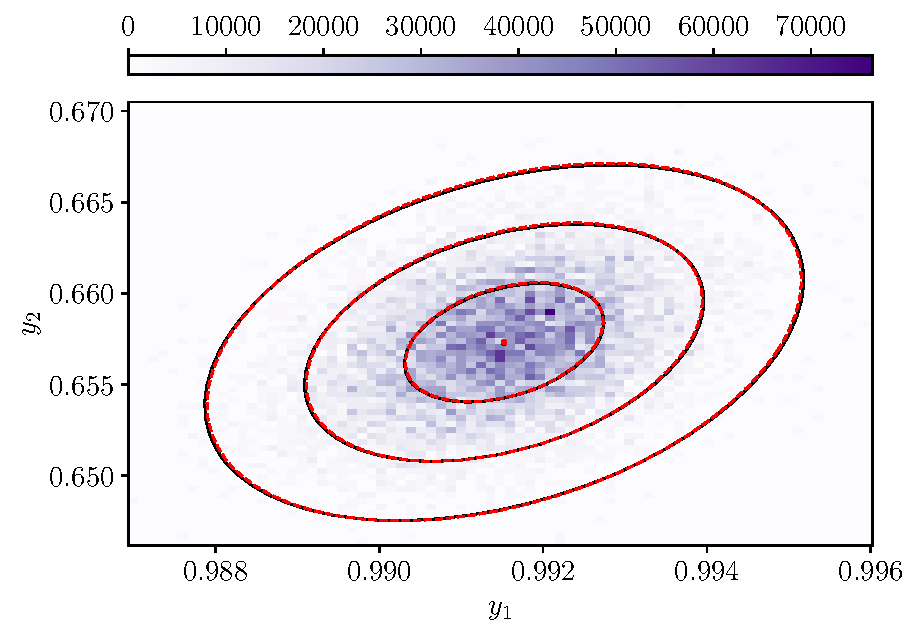
\includegraphics[width=\textwidth]{chp04_paper_numerics/figures/rossby/hist_0.001.pdf}
			\caption{\(\epsilon = 10^{-3}\)}
			\label{fig:y_hists_d}
		\end{subfigure}
		\caption{Histograms of \(y_t^{(\epsilon)}\) from direct simulation of \eqref{eqn:sde_y}, for four different \(\epsilon\) values.
		Overlaid in black are contours of the Gaussian solution \eqref{eqn:linear_gauss_sol} of the linearised SDE \eqref{eqn:linear_sde_inform}, which correspond to the first three standard deviation levels centred at the mean \(F_0^t(x)\).
        In dashed blue are corresponding contours computed from the sample covariance matrix of the realisations.
        }
		\label{fig:y_hists}
	\end{center}
\end{figure}
For \(r = 1,2,3,4\), \(E_r\!\left(\epsilon\right)\) is shown (in a logarithmic scale) for decreasing values of \(\epsilon\) in \Cref{fig:gamma_z_valid}.
\Cref{thm:main} predicts that \(\log_{10}\left(E_r\!\left(\epsilon\right)\right)\) should decay linearly with a slope greater than \(2r\) as \(\epsilon\) decreases to zero.
The lines of best fit for each value of \(r\) in \Cref{fig:gamma_z_valid} show this behaviour, and are therefore consistent with \Cref{thm:main}.

\begin{figure}
	\begin{center}
		\begin{subfigure}{0.49\textwidth}
			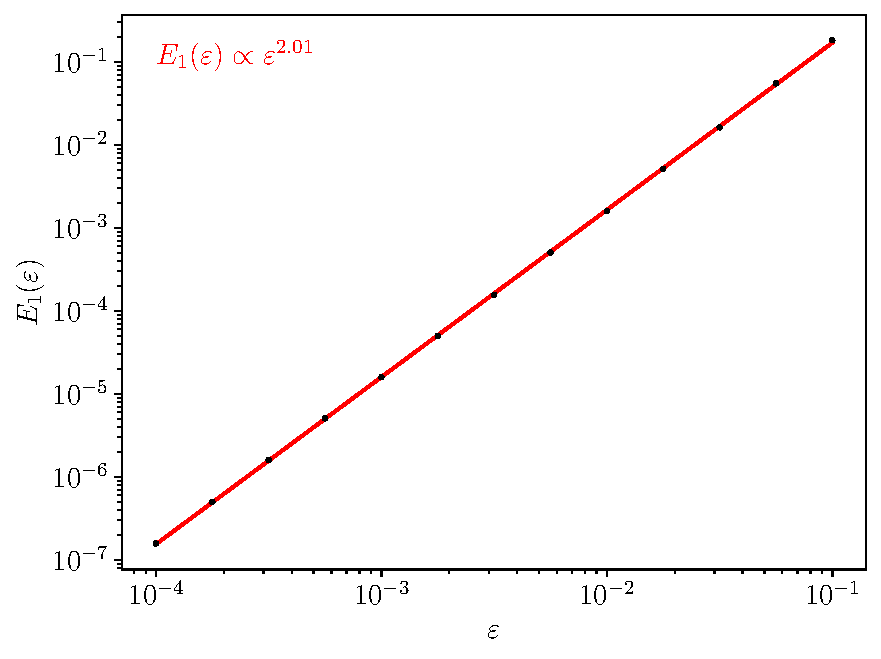
\includegraphics[width=\textwidth]{chp04_paper_numerics/figures/rossby/str_err_r_1.0.pdf}
			\caption{\(r = 1\) (mean)}
			\label{fig:gamma_z_valid_1}
		\end{subfigure}
\begin{subfigure}{0.49\textwidth}
			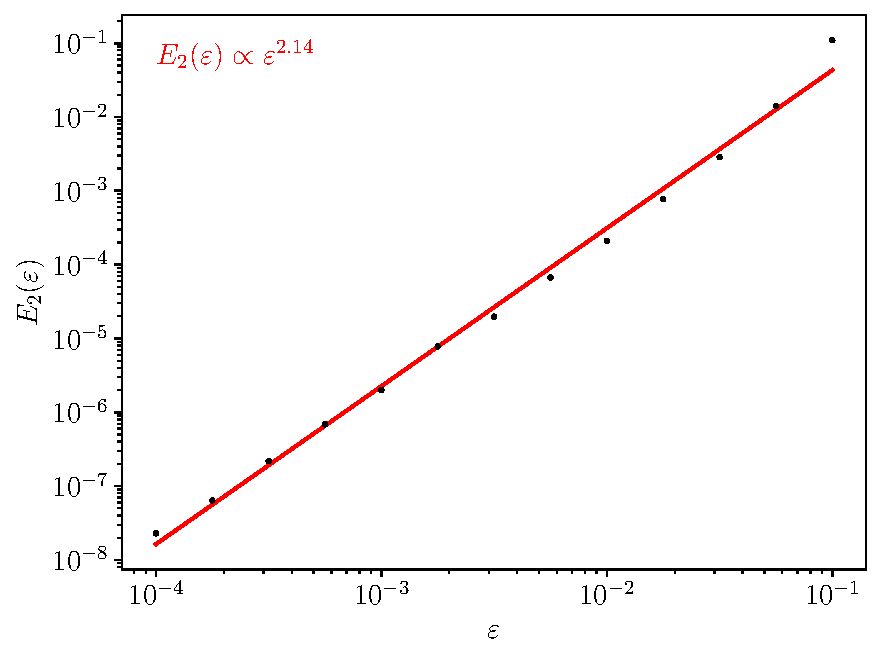
\includegraphics[width=\textwidth]{chp04_paper_numerics/figures/rossby/str_err_r_2.0.pdf}
			\caption{\(r = 2\) (variance)}
			\label{fig:gamma_z_valid_2}
		\end{subfigure}
		\begin{subfigure}{0.49\textwidth}
			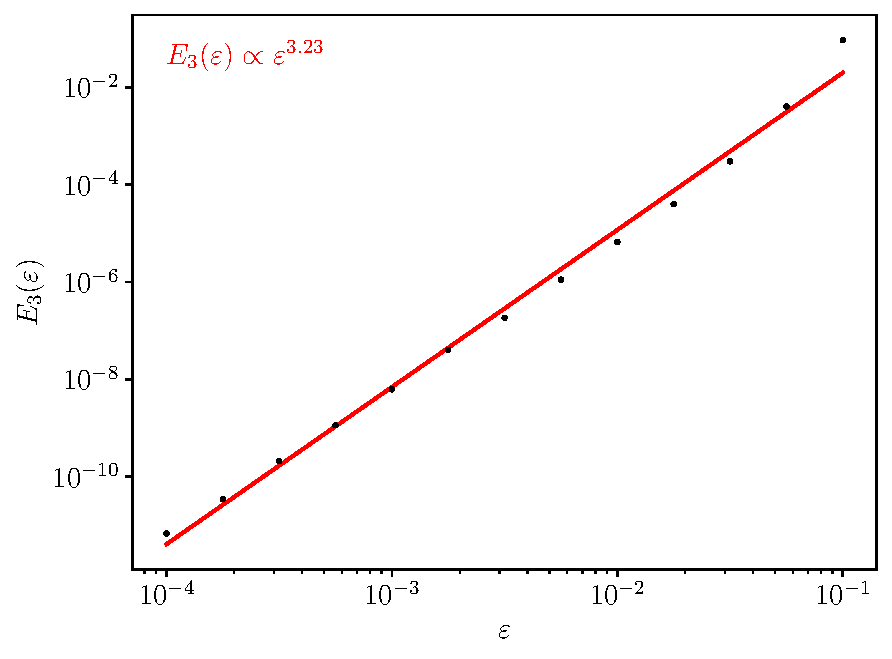
\includegraphics[width=\textwidth]{chp04_paper_numerics/figures/rossby/str_err_r_3.0.pdf}
			\caption{\(r = 3\) (skewness)}
			\label{fig:gamma_z_valid_3}
		\end{subfigure}
		\begin{subfigure}{0.49\textwidth}
			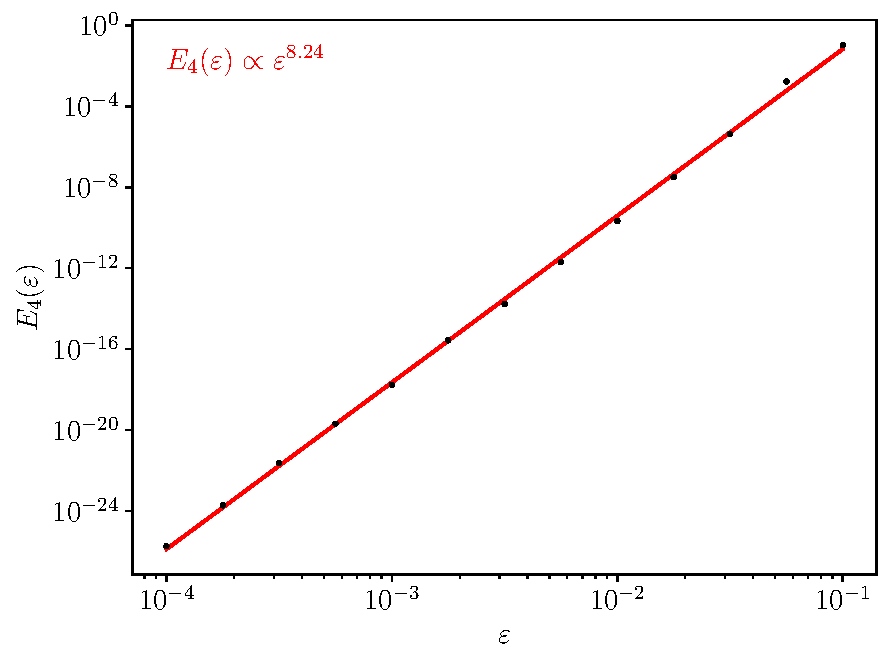
\includegraphics[width=\textwidth]{chp04_paper_numerics/figures/rossby/str_err_r_4.0.pdf}
			\caption{\(r = 4\) (kurtosis)}
			\label{fig:gamma_z_valid_4}
		\end{subfigure}

		\caption{Validation of \Cref{thm:main}, by plotting the sample \(r\)th raw moment distance (the error metric \(\Gamma_z^{(r)}(\epsilon)\)) between \(10000\) realisations of \(z_t^{(\epsilon)}(x)\) and \(z_t(x)\), for decreasing values of \(\epsilon\).
        A line of best fit (in red) is placed on each, and the resulting slope indicated.}
		\label{fig:gamma_z_valid}
	\end{center}
\end{figure}
